\documentclass[conference]{IEEEtran}
\IEEEoverridecommandlockouts
\usepackage{cite}
\usepackage{amsmath,amssymb,amsfonts}
\usepackage{algorithm}
\usepackage{algpseudocode}
\usepackage{amsfonts} % 用于支持 \mathbb{N}
\usepackage{graphicx}
\usepackage{textcomp}
\usepackage{xcolor}
\usepackage{booktabs}
\usepackage{multirow}
\usepackage{array}
\usepackage{siunitx}
\sisetup{mode = text}
\usepackage[hidelinks]{hyperref}
\def\BibTeX{{\rm B\kern-.05em{\sc i\kern-.025em b}\kern-.08em
    T\kern-.1667em\lower.7ex\hbox{E}\kern-.125emX}}

\graphicspath{{figures/}}

\begin{document}

\title{Split-Path ML-Augmented Prefetching: Low-Latency Storage Architecture for EVM State}
% \title{SPLIT: Split-Path Learned Inference Table for EVM State}

\author{\IEEEauthorblockN{Tianyu Mao, Junqin Huang$^{*}$, Xinming Shu, Linghe Kong, Guihai Chen}
\IEEEauthorblockA{\textit{School of Computer Science},
\textit{Shanghai Jiao Tong University}, Shanghai, China\\
\{mist123,junqin.huang,Xinming\_Shu,linghe.kong,chen-gh\}@sjtu.edu.cn}
% \and
% \IEEEauthorblockN{Second Author$^{2}$}
% \IEEEauthorblockA{\textit{Dept. of Computer Science}\\
% \textit{University Name}\\
% City, Country \\
% email@example.com}
\thanks{$^{*}$Junqin Huang is the corresponding author.}
}

\maketitle

\begin{abstract}
The Ethereum Virtual Machine (EVM) acts as the core runtime for blockchain smart contracts, where cold storage slot access becomes a severe I/O bottleneck restricting transaction throughput. We profile storage latency on Erigon, a mainstream high-performance Ethereum execution client optimized with flat state storage and fast sync mechanisms, and observe a massive performance gap: cold storage loads take roughly \qty{3}{\micro\second}, 100$\times$ slower than hot hits in the intra-block cache (\qty{30}{\nano\second}). Unfortunately, the first access to any storage slot within a block is always a cold load, amplifying this overhead. Two dominant prefetching approaches suffer inherent flaws: static rule tables deliver $O(1)$ lookup latency but fail to adapt to dynamic contract invocation patterns, while online Machine Learning (ML) prefetchers introduce unaffordable inference overhead that exceeds latency savings by three orders of magnitude.
To bridge the gap, we propose a split-path ML-augmented prefetch architecture for EVM state storage, fully decoupling ML inference from the latency-sensitive online critical path. The online path maintains a lightweight hash table indexed by $(to, selector)$ pairs to realize constant-time lookups, while the offline path periodically trains a multi-label classification model on historical transaction traces to generate incremental prefetch patterns. After dedicated filtering, refined patterns are merged into the online hash table to continuously boost prefetch coverage. 
Trace-driven evaluations over 1,001 consecutive Ethereum mainnet blocks containing nearly 94,000 transactions demonstrate that our design lifts prefetch recall from 22.23\% to 31.17\% (corresponding to a 40.2\% relative gain), cuts overall storage access overhead by 11.3\%, and delivers a 12.7\% speedup on EVM storage operations.
\end{abstract}

\begin{IEEEkeywords}
EVM State Access, Data Prefetching, Split-path Architecture, Intra-block Cache.
\end{IEEEkeywords}


\section{Introduction}

% Ethereum is the most widely deployed smart contract platform, hosting thousands of decentralized applications. The Ethereum Virtual Machine (EVM) serves as Ethereum's core execution engine, which executes smart contract bytecode. Among all EVM operations, storage access (\textit{i.e.}, \texttt{SLOAD/SSTORE}) is the dominant performance bottleneck. The Ethereum Improvement Proposal EIP-7707~\cite{eip7707} notes that data loading accounts for over 70\% of block execution time in some clients. This is fundamentally because storage is the only operation that requires database I/O. All other EVM operations (\textit{e.g.}, arithmetic, memory, control flow) are mainly compute-bound and operate at nanosecond latency.

Ethereum stands as the most widely adopted smart contract platform, supporting thousands of decentralized applications (dApps). As the core execution component of Ethereum, the Ethereum Virtual Machine (EVM) is responsible for executing smart contract bytecode. Among all EVM instructions, storage access operations (\textit{i.e.}, \texttt{SLOAD/SSTORE}) constitute the primary performance bottleneck for blockchain execution. Ethereum Improvement Proposal (EIP) 7707~\cite{eip7707} highlights that data loading operations consume over 70\% of the block execution time in certain Ethereum clients. This performance disparity stems fundamentally from the fact that storage access is the only EVM operation that involves disk database I/O. In contrast, other EVM operations, including arithmetic computation, memory manipulation, and control flow execution, are predominantly compute-bound and feature nanosecond-level execution latency.

% A storage slot is the basic unit of persistent state in Ethereum. It is uniquely identified by a contract address and a 256-bit storage key. The EVM distinguishes two types of storage access: \emph{hot} accesses that hit a cache within the same block, and \emph{cold} accesses that require loading data from the database. We measured these two access modes on our hardware platform and found that hot access completes in approximately 30~ns, while cold access requires approximately 3~$\mu$s. This represents a roughly 100$\times$ latency gap. The first access to any storage slot within a block is always a cold access, which constitutes the fundamental performance bottleneck. Based on traces from 94,463 Ethereum mainnet transactions (about 1,000 blocks), a transaction accesses 16.2 storage slots on average, of which 12.3 are first accesses within a block. Cold accesses account for 76\% of all storage slot access events. The unexpectedly high ratio indicates that most slots are accessed by only one transaction per block: 87.9\% of storage slots appear in exactly one transaction within their block. % Computed from 94,463 txs: 1,160,174 unique (slot, block) pairs, of which 1,019,326 (87.9%) appear in only 1 tx per block. This makes the cold access problem both severe and difficult to mitigate through intra-block caching alone.

A storage slot is the fundamental unit of persistent state in Ethereum, uniquely determined by the combination of a contract address and a 256-bit storage key. The EVM categorizes storage accesses into two types: \emph{hot} accesses that hit the in-block cache, and \emph{cold} accesses that fetch data directly from the underlying database. We benchmarked both access patterns on our hardware platform, yielding a measured latency of approximately \qty{30}{\nano\second} for hot accesses and \qty{3}{\micro\second} for cold accesses, corresponding to a nearly 100$\times$ performance gap. Notably, the first access to any storage slot within a block is inherently a cold access, which becomes a critical performance bottleneck for block execution. We further evaluate real-world storage access characteristics using transaction traces collected from 94,463 Ethereum mainnet transactions across around 1,000 blocks. The experimental results show that each transaction accesses an average of 16.2 storage slots, among which 12.3 correspond to in-block first-time accesses. Overall, cold accesses occupy 76\% of all storage access events. This high proportion suggests that most storage slots are accessed sparsely within a single block. Specifically, 87.9\% of storage slots are touched by exactly one transaction per block.

% Fig.~\ref{fig:evm_workflow} illustrates the EVM execution workflow and the role of storage access. A pending transaction enters the EVM for bytecode execution. A hot access returns the value from the cache immediately, while a cold access triggers a database lookup, which is then loaded into the cache for subsequent accesses. The Erigon client~\cite{erigon} optimizes storage access through an intra-block state caching mechanism. It caches state within a block boundary to accelerate hot accesses. However, even with such optimizations, cold accesses still require a full database load.

\begin{figure}[t]
\centering
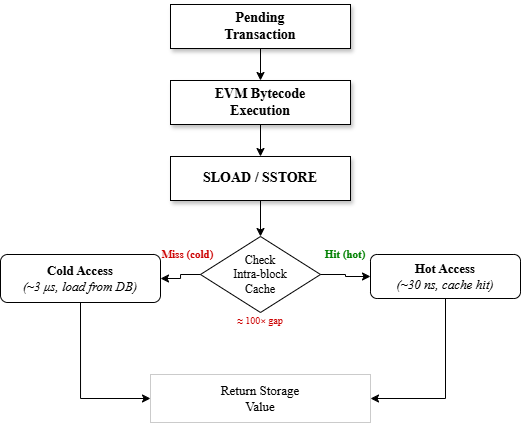
\includegraphics[width=0.9\columnwidth]{figures/evm_workflow.pdf}
\caption{The cold and hot storage access paths in the EVM.}
\label{fig:evm_workflow}
\vspace{-0.3cm}
\end{figure}

Fig.~\ref{fig:evm_workflow} visualizes the overall EVM execution workflow and highlights the pivotal role of storage access during transaction processing. Pending transactions are submitted to the EVM for bytecode interpretation and execution. For storage operations, hot accesses instantly return cached state data, whereas cold accesses necessitate explicit database queries, with the loaded data subsequently buffered in the cache to serve subsequent in-block accesses. The Erigon client~\cite{erigon} optimizes storage latency by adopting an intra-block state caching strategy, which caches state data within a single block to expedite hot access operations. Despite such optimization efforts, cold accesses still incur unavoidable full database loading overhead.

% The severity of this bottleneck demands an effective optimization strategy. Inspired by CPU cache prefetching~\cite{primer_prefetch}, a natural optimization approach is to pre-load the required storage slots into the cache before transaction execution, converting cold accesses into hot accesses, i.e., prefetching. Existing prefetching approaches fall into two categories. The first is static rule tables. These use a hash table indexed by pattern keys, achieving O(1) lookup with zero inference overhead. However, their coverage is insufficient for dynamic workloads. Rules become stale when contracts are upgraded or call patterns change. The second category is online Machine Learning (ML) methods~\cite{survey_prefetch}, which can capture complex, dynamic patterns. However, their inference latency poses a fundamental challenge. A single inference of our LightGBM multi-label classification model takes approximately 28~ms on the evaluation platform (Section~\ref{sec:experiment-configuration}), while a single prefetch saves at most 3~$\mu$s. This is a huge gap of approximately three orders of magnitude.

The severity of this bottleneck calls for effective optimization strategies. Inspired by CPU cache prefetching~\cite{primer_prefetch}, a straightforward optimization preloads required storage slots into cache prior to transaction execution to convert cold accesses into hot ones, namely prefetching. Existing prefetching schemes fall into two categories. The first adopts static rule tables: hash tables indexed by pattern keys with $O(1)$ lookup complexity, yet offering limited coverage for dynamic workloads. Rules turn obsolete once contracts upgrade or call patterns shift. The second group consists of online Machine Learning (ML) methods~\cite{survey_prefetch}, capable of capturing intricate dynamic patterns but hindered by heavy inference latency. On our evaluation platform (see Section~\ref{sec:experiment-configuration}), one inference pass of our LightGBM multi-label classifier consumes roughly \qty{28}{\milli\second}, whereas each prefetch only cuts up to \qty{3}{\micro\second} of latency, which is a massive gap spanning three orders of magnitude.

% To formalize this problem, we introduce the coverage parameter $\alpha$ ($0 \leq \alpha \leq 1$). It represents the fraction of transaction execution time that can overlap with ML inference. We define the effective inference overhead as $\text{Overhead}_{\text{eff}} = \max(0, t_{\text{pred}} - \alpha \cdot t_{\text{exec}})$, where $t_{\text{pred}}$ is the total ML inference time and $t_{\text{exec}}$ is the total transaction execution time. Even under the ideal assumption of $\alpha = 1.0$ (100\% parallel coverage), $t_{\text{pred}}$ (14.78~s) exceeds the storage cost savings (0.005~s). Fig.~\ref{fig:alpha} visualizes the relationship. We conclude that online ML inference is quantitatively infeasible for EVM storage prefetching. This negative result is the fundamental motivation for our work.

To rigorously formalize this problem, we introduce the coverage parameter $\alpha \in [0,1]$, the fraction of transaction execution time that can overlap with ML inference. We define the effective inference overhead as $\text{Overhead}_{\text{eff}} = \max(0, t_{\text{pred}} - \alpha \cdot t_{\text{exec}})$, where $t_{\text{pred}}$ denotes the total ML inference time and $t_{\text{exec}}$ denotes the total transaction execution time. Even under the ideal case of $\alpha = 1.0$, $t_{\text{pred}}$ (\qty{14.78}{\second}) significantly exceeds the storage cost savings (\qty{0.005}{\second}). Fig.~\ref{fig:alpha} visualizes the above relationship. We conclude that online ML inference is quantitatively infeasible for EVM storage prefetching. This negative finding serves as the core motivation for our work.

% 这张图来自脚本 evm_analysis/viz/plot_sim_figures.py，如果需要修改图片，请去这个脚本里面修改。
\begin{figure}[t]
\centering
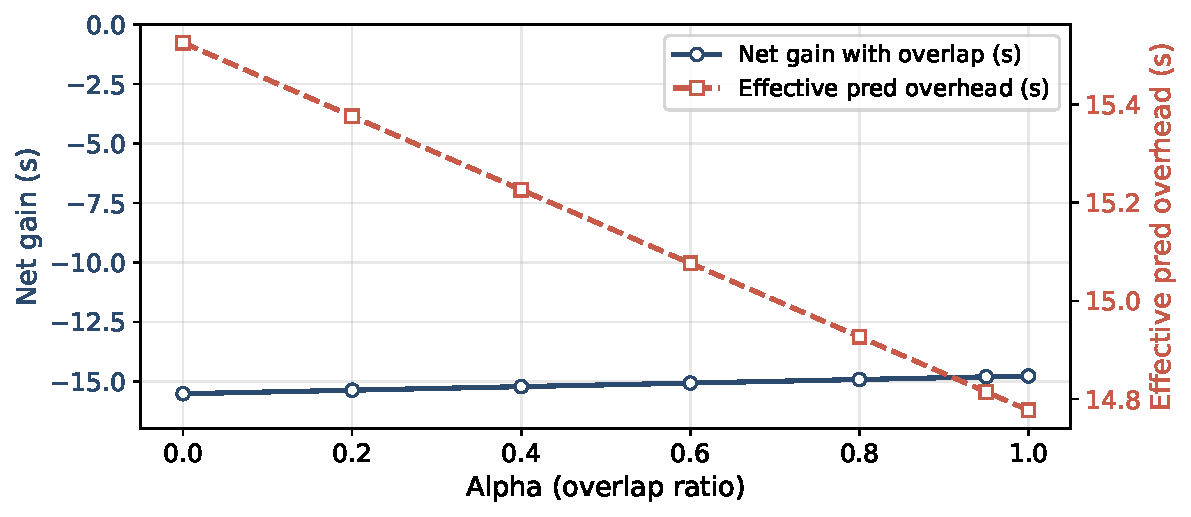
\includegraphics[width=\columnwidth]{figures/fig_alpha.pdf}
\caption{The effective inference overhead under varying $\alpha$ values, compared to the potential storage access cost savings.}
\label{fig:alpha}
\vspace{-0.3cm}
\end{figure}

%（已删除） The broader EVM optimization landscape~\cite{survey_prefetch} encompasses client-level storage layout improvements, protocol-level access lists, static analysis techniques, and parallel execution models. These works are orthogonal to prefetching. For ML-based prefetching, prior works have explored online classification models trained on historical access patterns. While effective at capturing complex correlations, all existing approaches place ML inference on the critical execution path. In contrast, our approach fundamentally differs by removing ML inference from the online path entirely.

% We propose \textbf{Split-Path ML-Augmented Prefetching} (SPML-PF), a novel architecture whose core insight is to decouple ML inference from online execution through an online/offline split-path design. In the \emph{online path}, a hash table indexed by pattern keys (\emph{to}, \emph{selector}), i.e., the target contract and function identifier, performs O(1) lookups with zero ML overhead. The \emph{offline path} runs a classification model on historical transaction data in batch. It generates incremental patterns that are merged into the online hash table.  Because the incremental patterns adopt the same key-value format as the existing entries, merging them preserves the O(1) lookup efficiency while continuously expanding the hash table with newly discovered access patterns. Our contributions are summarized as follows:
% \begin{itemize}
%     \item \textbf{Problem identification.} Through execution time coverage analysis, we quantitatively prove that online ML approaches are infeasible for EVM storage prefetching. The effective overhead exceeds potential savings by approximately three orders of magnitude.
%     \item \textbf{SPML-PF design.} We propose an online/offline split-path hybrid prefetching architecture that removes ML inference from the critical execution path while maintaining O(1) online lookup efficiency.
%     \item \textbf{Empirical evaluation.} On 1,001 consecutive Ethereum mainnet blocks (approximately 94K transactions), our method achieves 40.2\% relative recall improvement and 11.3\% storage access cost reduction.
% \end{itemize}

In this paper, we propose \textbf{Split-Path ML-Augmented Prefetching} (SPML-PF), a novel architecture that decouples ML inference from online execution via a dedicated online/offline split-path design. The \emph{online path} uses a hash table indexed by pattern keys $(to, selector)$, namely the target contract address and function identifier, for $O(1)$ lookups with zero runtime ML overhead. The \emph{offline path} executes a classification model over historical transaction data in batch, producing incremental access patterns that are merged into the online hash table. Since these incremental patterns follow the same key-value format as existing entries, the merged hash table retains $O(1)$ lookup efficiency while progressively enriching the pattern library. Our main contributions are summarized as follows:
\begin{itemize}
    \item \textbf{Problem identification.} Through quantitative execution coverage analysis, we demonstrate that online ML-based prefetching is infeasible for EVM storage optimization, as the incurred inference overhead exceeds the achievable performance savings by nearly three orders of magnitude.
    \item \textbf{SPML-PF design.} We present a hybrid online/offline split-path prefetching framework that eliminates ML inference from the critical execution path while preserving $O(1)$ online lookup efficiency.
    \item \textbf{Empirical evaluation.} Evaluated on 1,001 consecutive Ethereum mainnet blocks (roughly 94K transactions), our approach achieves a 40.2\% relative recall improvement and an 11.3\% reduction in storage access overhead.
\end{itemize}

\section{Related Work}
\label{sec:related-work}

We survey prior work along three dimensions: EVM storage access optimizations, data prefetching mechanisms, and learned index designs, and highlight the orthogonality and novelty of our proposed approach.

\subsection{EVM Storage Access Optimization}
\label{sec:evm-storage-opt}
% 按"执行栈四层次"组织：存储引擎层 → 交易接口层 → 字节码分析层 → 执行调度层
% 叙事主线：四个层次覆盖不同优化维度，都与我们正交；没有任何一个从 prefetching 角度解决问题

Research on EVM storage efficiency targets four execution-stack layers. At the storage engine layer, Storage Replica~\cite{storage_replica} uses a flat-trie hybrid, achieving a 6$\times$ speedup. At the transaction interface layer, EIP-2930~\cite{eip2930}, EIP-7650~\cite{eip7650}, and EIP-7863~\cite{eip7863} add explicit access lists or block-level warming, but require the caller to declare slots in advance. At the bytecode analysis layer, static analysis identifies redundant accesses~\cite{needless_writes,evmtracer,evmshield}; EVMTracer~\cite{evmtracer} reports 34.97\% of storage loads are redundant. At the execution scheduling layer, parallel frameworks~\cite{ostm,reddio,conflict_spec} improve throughput via transactional memory or pipelined execution, achieving up to 3.91$\times$ speedup. None addresses predictive prefetching, making all four orthogonal to our work.

\subsection{Data Prefetching}
\label{sec:data-prefetching}
% 四个层次：传统分类 → ML 效率进化 → RL 自适应 → FarSight → EVM 不可行性

% Existing data prefetching technologies span next-line, stride, spatial, and temporal predictors~\cite{primer_prefetch,survey_prefetch,markov_prefetch}, and extends to distributed deep learning caches~\cite{nas_paper_1} and solid-state drive optimization~\cite{nas_paper_2}.

Data prefetching technologies cover a rich set of predictors, including next-line, stride, spatial, and temporal schemes~\cite{primer_prefetch,survey_prefetch,markov_prefetch}, and have been further extended to distributed deep learning caches~\cite{nas_paper_1} and solid-state drive optimization~\cite{nas_paper_2}.

Recent ML prefetchers focus on efficient architectures. Voyager~\cite{voyager} uses a hierarchical neural network separating page-level and offset-level prediction, achieving 41.6\% IPC improvement. The efficient neural prefetcher~\cite{efficient_neural} achieves 60\% IPC improvement on SPEC~2006 while reducing MACs by 15.4$\times$ and parameters by 6.7$\times$. A$^2$P~\cite{a2p} adopts an attention mechanism with bitmap labeling, achieving 18.4\% IPC improvement on GAP. Beyond static architectures, reinforcement learning introduces adaptivity: Pythia~\cite{pythia} achieves 3.4--20.2\% improvement over prior methods, and RL-CoPref~\cite{rlcopref} coordinates multiple prefetchers for 35.5\% IPC improvement.

FarSight~\cite{farsight} is architecturally closest to our approach. It separates offline training from online inference, achieving 3.6$\times$ speedup for far-memory access, but still places a neural network on the critical inference path.

Despite architectural diversity, all ML-based prefetchers place inference on the online path. In the CPU context this is acceptable as the cost amortizes across many cache misses. In the EVM context, however, a single inference takes approximately \qty{28}{\milli\second} while each cold access saves at most \qty{3}{\micro\second}. This three-order-of-magnitude gap makes online ML infeasible and motivates our split-path design.

\subsection{Learned Indexes}
\label{sec:learned-indexes}
% 瓶颈维度（ALEX/PGM/RadixSpline）→ 混合架构（Shift-Table）→ 范式推广

Learned indexes replace traditional structures with ML models that predict data positions. ALEX~\cite{alex} targets updates with gapped arrays, achieving 4.1$\times$ speedup over B+-tree. PGM~\cite{pgm} provides worst-case guarantees via piecewise linear regression, achieving 83$\times$ space reduction. RadixSpline~\cite{radixspline} optimizes construction through single-pass learning. Shift-Table~\cite{shifttable} combines an ML model with an algorithmic correction layer for 1.5--2$\times$ speedup, a hybrid design that aligns with our split-path architecture. 

To the best of our knowledge, this is the first work to apply ML-augmented prefetching to EVM storage optimization. We address EVM storage efficiency from a prefetching angle, which is orthogonal to all existing EVM optimizations. Our online/offline split-path design removes ML inference entirely from the critical execution path, unlike all prior ML prefetchers. We apply the ML-augmented data structure paradigm, previously explored for database indexes, to the domain of EVM storage slot prefetching.

\section{Preliminary}
\label{sec:preliminary}

This section introduces the EVM storage model, the concept of pattern keys, and the
prefetching opportunity they enable. It also formulates the prediction problem solved in
this paper.

\subsection{EVM Storage Model}
\label{sec:evm-storage}

The Ethereum Virtual Machine maintains a world state as a Merkle Patricia Trie (MPT).
Each smart contract has its own private storage space. This space is a key-value mapping
from 256-bit storage keys to 256-bit values. A single entry in this mapping is called a
\textit{storage slot}. Each slot is uniquely identified by a
\texttt{(contract\_address}, \texttt{storage\_key)} pair. Smart contracts read and write
these slots through two EVM opcodes: \texttt{SLOAD} (read) and \texttt{SSTORE} (write).

Erigon, a popular Ethereum execution client, introduces an \textit{intra-block state}
cache to accelerate repeated slot accesses within the same block~\footnote{Erigon
intra-block state implementation:
\url{https://github.com/erigontech/erigon/blob/main/execution/state/intra_block_state.go}}.
This cache is cleared at the start of each new block.
When a transaction accesses a storage slot, Erigon first checks this cache. If the slot
is already present, it is a \textit{hot access} and the read completes in approximately
\qty{30}{\nano\second}. If it is not present, it is a \textit{cold access} and Erigon reads the slot from
the underlying database at approximately \qty{3}{\micro\second}.
The cold access problem follows directly from this design. The first access to any
storage slot within a block is always a cold access, so contract invocations that touch
many unique slots are dominated by cold accesses. A Uniswap V2 swap
transaction~\cite{uniswapv2}, for instance, may touch 10 to 50 unique storage slots, each incurring a
cold access at \qty{3}{\micro\second}. The total storage loading time is 30 to \qty{150}{\micro\second} per
transaction and grows linearly with the number of unique slots accessed.

\subsection{Pattern Keys and Prefetching Opportunity}
\label{sec:pattern-keys}

A \textit{pattern key} is a two-tuple $(to, selector)$. Here $to$ is the target
contract address, and $selector$ is the four-byte function selector extracted from the
transaction's calldata. Transactions that call the same contract function share the same
pattern key, which makes pattern keys a natural grouping mechanism for storage
access prediction.

Transactions with the same pattern key tend to access similar sets of storage slots.
The union set of a pattern key $k$ is defined as

\begin{equation}
U(k) = \bigcup_{tx \in T(k)} S_{\text{actual}}(tx),
\label{eq:union-size}
\end{equation}
where $T(k)$ is the set of all transactions with pattern key $k$, and
$S_{\text{actual}}(tx)$ is the set of storage slots accessed during the execution of
transaction $tx$. The union size $|U(k)|$ measures the storage access complexity of a
calling pattern: small values indicate a stable and repeatable set of slots. In our
dataset (see Section~\ref{sec:evaluation}), over 80\% of pattern keys have a union size
of fewer than 50 slots. This stability creates a clear prefetching opportunity. If we can
determine the pattern key of a pending transaction before execution and have recorded the
storage slots historically associated with that key, we can pre-load those slots into the
intra-block cache. Every pre-loaded slot becomes a hot access instead of a cold access,
saving approximately \qty{3}{\micro\second} per slot.

\subsection{Problem Formulation}
\label{sec:problem-formulation}

We formalize the EVM storage slot prefetching problem as constructing a pattern table $\mathcal{H}$ that maps each pattern key to a predicted storage slot set for online lookup.

\textbf{Input.} Historical transaction traces with recorded execution information. For each transaction $tx$:
\begin{itemize}
    \item The pattern key $\kappa(tx) = (tx.to, tx.selector)$ is known before execution,
    \item The ground-truth accessed slot set $S_{\text{actual}}(tx)$ is extracted from execution traces.
\end{itemize}

\textbf{Output.} A pattern table $\mathcal{H}$ that maps each key $k$ to a storage slot set $\mathcal{H}[k]$. During online execution, each pending transaction $tx$ retrieves its predicted set by a single lookup:
\[
S_{\text{pred}}(tx) = \mathcal{H}[\kappa(tx)].
\]

\textbf{Objective.} Over the evaluation dataset, the table is evaluated by aggregate recall and precision:

\begin{align}
\text{Recall} &= \frac{\sum_{tx} |S_{\text{pred}}(tx) \cap S_{\text{actual}}(tx)|}
                 {\sum_{tx} |S_{\text{actual}}(tx)|}, \nonumber \\
\text{Precision} &= \frac{\sum_{tx} |S_{\text{pred}}(tx) \cap S_{\text{actual}}(tx)|}
                   {\sum_{tx} |S_{\text{pred}}(tx)|}. \label{eq:objective}
\end{align}

\begin{figure*}[t]
\centering
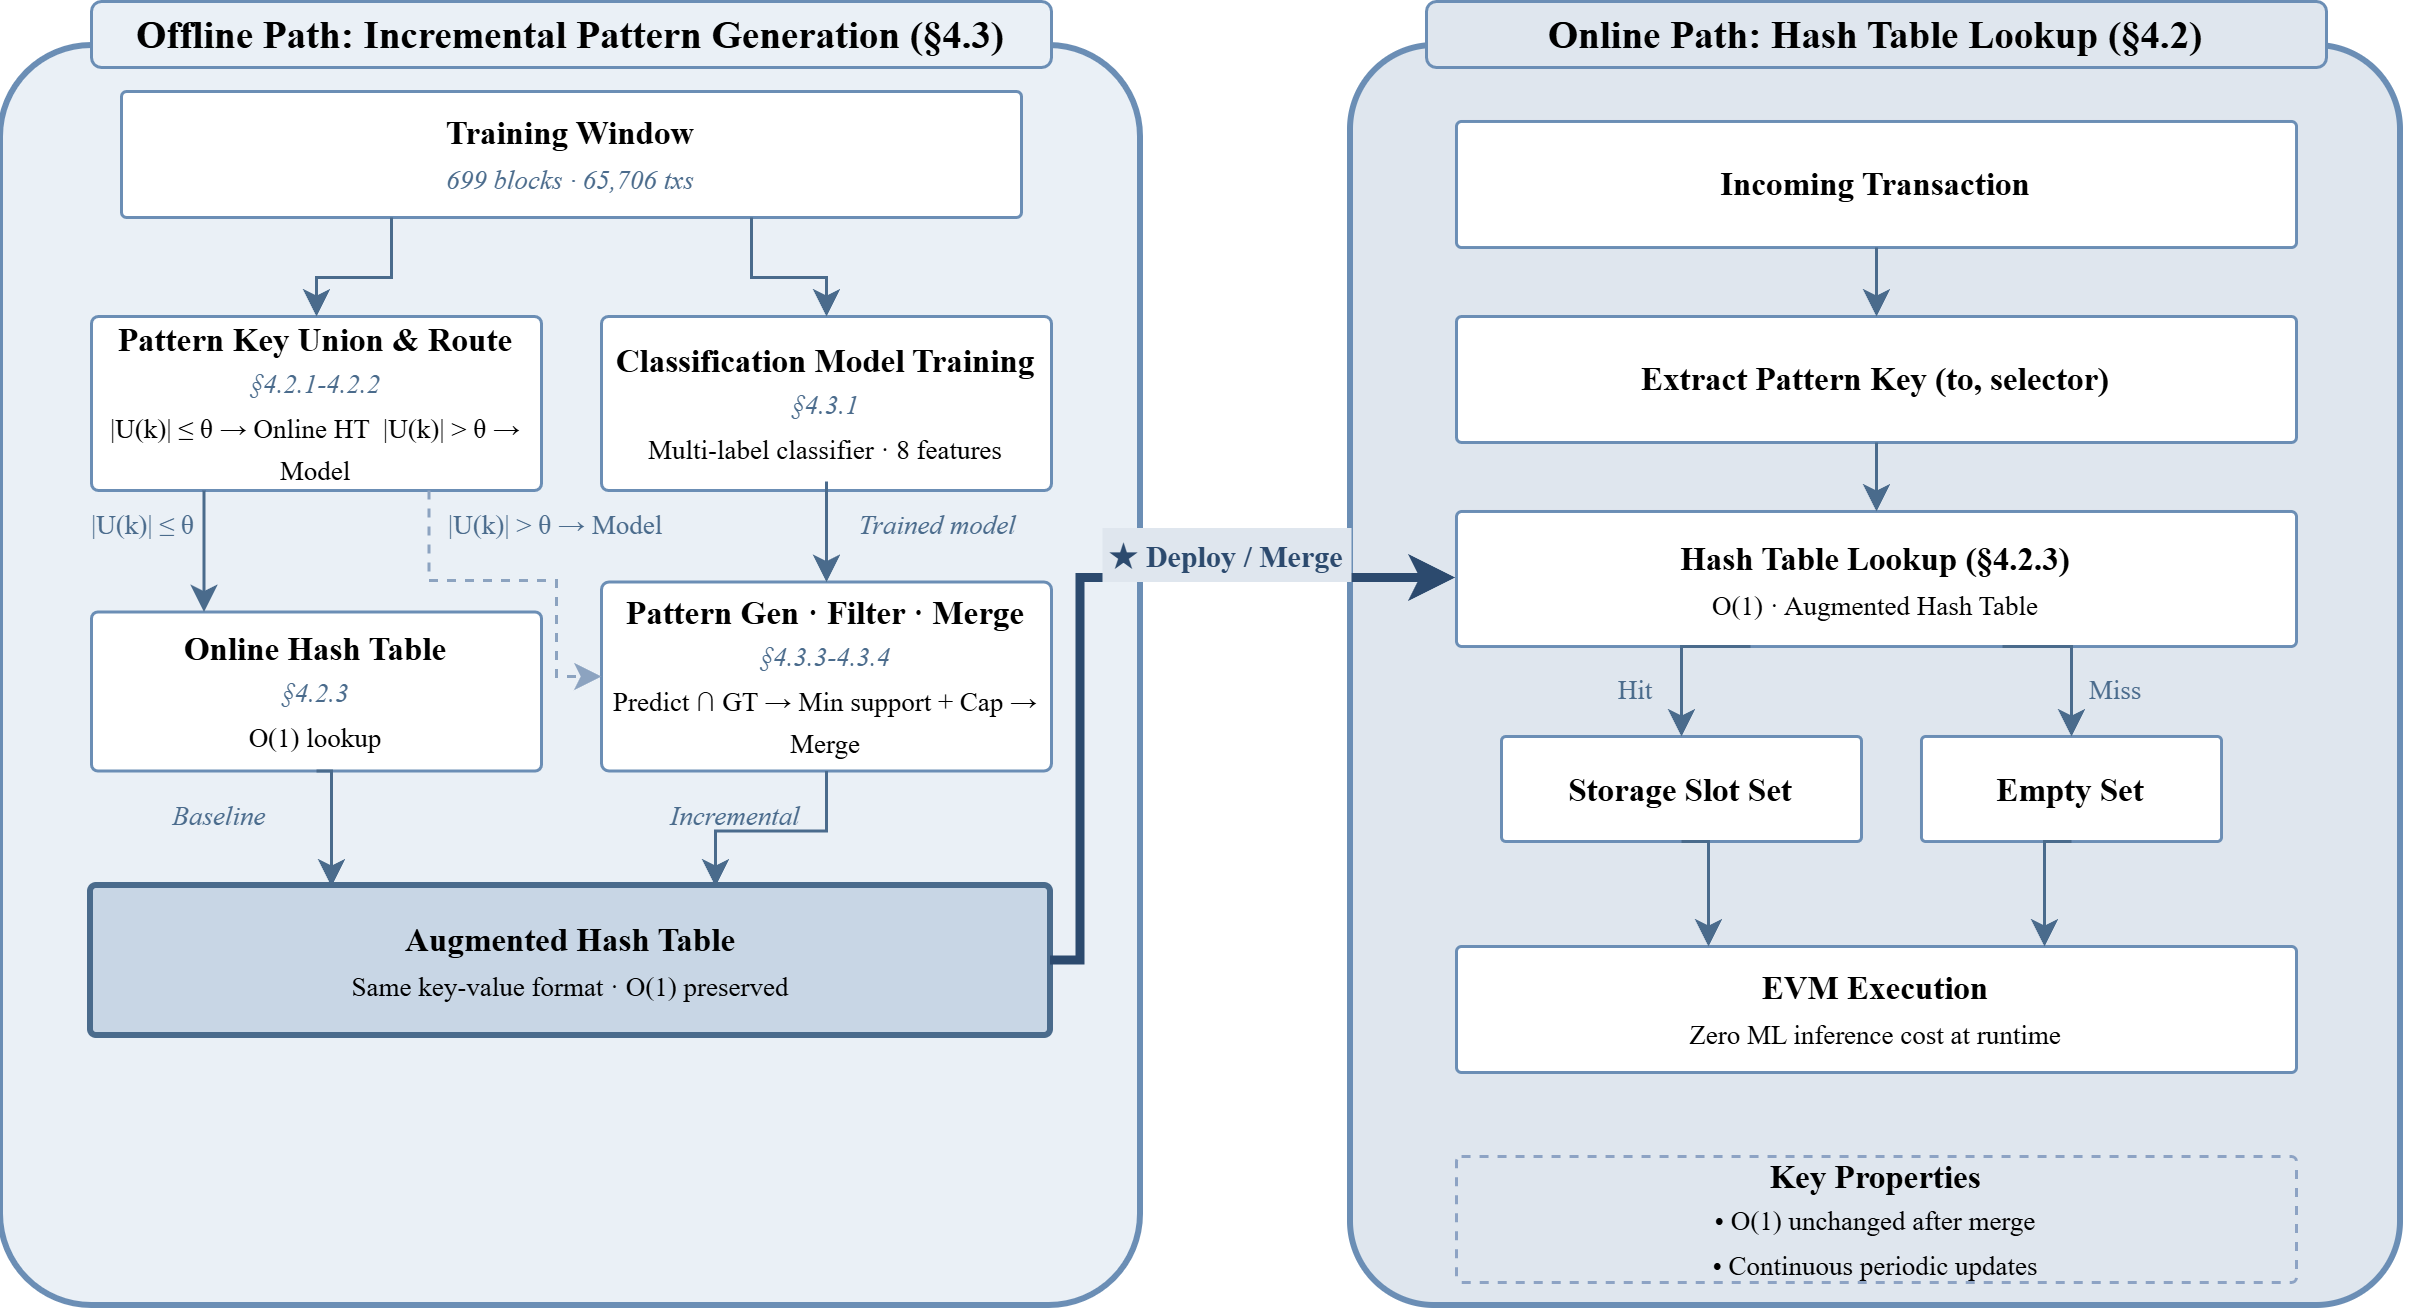
\includegraphics[width=0.95\textwidth]{system_design_architecture.pdf}
\caption{SPML-PF architecture overview.}
\label{fig:architecture}
%\vspace{-0.3cm}
\end{figure*}

\textbf{Constraint.} The lookup $\mathcal{H}[\kappa]$ must be $O(1)$ and incur zero ML inference overhead. All model inference is restricted to offline batch processing, separate from the online critical path.

\textbf{Distinction from Erigon.} The Erigon intra-block cache is \textit{passive}: it caches storage slots only after they are first accessed. Our approach is \textit{active}: we pre-load predicted slots before execution begins, converting correctly predicted cold accesses into hot accesses.

\section{System Design}
\label{sec:system-design}

We detail our split-path prefetching system in this section. We begin with a holistic overview of the architecture, followed by detailed descriptions of the online hash table lookup procedure and the offline pipeline for candidate accumulation, filtering and table augmentation.

% ---------------------------------------------------------------------------
% 4.1  Overview
% ---------------------------------------------------------------------------

\subsection{Overview}
\label{sec:overview}

The system adopts an online/offline split-path architecture that removes ML inference from the storage prefetching critical path. Fig.~\ref{fig:architecture} illustrates the overall workflow.

In the offline path, historical transaction traces are analyzed to discover storage access patterns. For each pattern key $(to, selector)$, the system aggregates the union of storage slots accessed across all transactions sharing that key. Keys with small union sizes are stored directly in a base hash table. Keys with large union sizes, which exhibit more complex access behavior, are routed to a classification model for selective per-transaction prediction. The model's predictions are compared against ground-truth access sets from the training window: correctly predicted (pattern key, slot) pairs accumulate a count, and pairs exceeding a threshold are merged into the hash table as augmented entries alongside the original base entries.

During online execution, each incoming transaction has its pattern key extracted and used to probe the augmented hash table. A hit returns the associated storage slot set for prefetching with zero ML inference overhead. A miss returns an empty set. Because the augmented entries share the same key-value format as the base table, the merge preserves $O(1)$ lookup efficiency. The pipeline supports continuous periodic updates on fresh data without modifying the online path.

% ---------------------------------------------------------------------------
% 4.2  Online Path: Hash Table Lookup
% ---------------------------------------------------------------------------
\subsection{Online Path: Hash Table Lookup}

\subsubsection{Pattern Key and Union Construction}
\label{sec:pattern-key}

As defined in Section~\ref{sec:pattern-keys}, a pattern key is a 2-tuple $(to, selector)$ used as the hash table lookup key.
During training, the system scans historical transactions and collects, for each pattern key, every storage slot accessed by any transaction with that key.
After deduplication, the resulting set is the \textbf{historical union}, whose size is $|U(k)|$ in Equation~\ref{eq:union-size}.
Small unions indicate deterministic access behavior suited to hash table storage, while large unions indicate complex patterns that are routed to the classification model.

\subsubsection{Threshold-based Routing}
\label{sec:threshold-routing}

A union threshold $\theta$ splits pattern keys into two groups: keys with $|U(k)| \leq \theta$ are stored in the online hash table and served via $O(1)$ lookup, while keys with $|U(k)| > \theta$ are routed to the classification model for selective per-transaction prediction and excluded from the hash table entirely.

This threshold addresses a fundamental trade-off. The hash table stores the complete union for each key. For small unions this approach is efficient because nearly every stored slot is likely to be needed. For large unions, storing the full set would introduce many irrelevant prefetches that waste cache bandwidth without improving recall. Routing those keys to the classification model avoids this problem, as the model produces selective predictions instead of returning the entire union. Conversely, routing all keys through the model would add unnecessary computation for the majority of keys whose behavior is already well captured by simple union storage.
Fig.~\ref{fig:cdf} shows the Cumulative Distribution Function (CDF) of union sizes per pattern key, with over 80\% of pattern keys having union sizes below 50, confirming that a modest threshold covers most keys efficiently.


% 绘图脚本: evm_analysis/viz/plot_figures.py / plot_figure1a_union_cdf()
\begin{figure}[t]
\centering
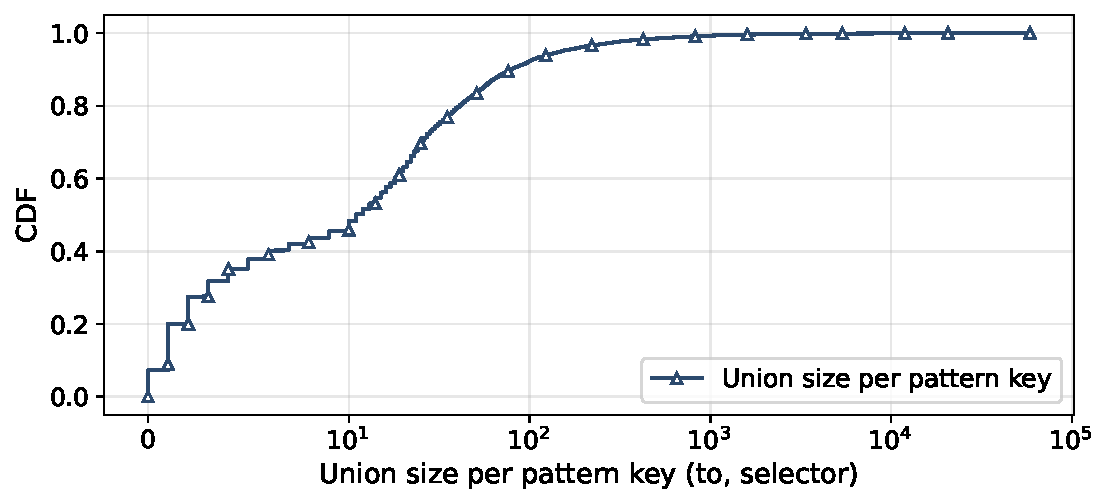
\includegraphics[width=\columnwidth]{figures/fig_cdf.pdf}
\caption{The CDF of union sizes per pattern key.}
\label{fig:cdf}
%\vspace{-0.5cm}
\end{figure}

The key advantage is that deterministic access patterns are served with zero inference overhead, while complex patterns are modeled offline without affecting online latency.

\subsubsection{Online Lookup}
\label{sec:online-lookup}

For each pending transaction, the system extracts its pattern key $(to, selector)$ and probes the online hash table in constant time, returning the associated storage slot set for prefetching on a hit and an empty set on a miss. The online path incurs zero ML inference cost.

% ---------------------------------------------------------------------------
% 4.3  Offline Path: Incremental Candidate Merging
% ---------------------------------------------------------------------------
\subsection{Offline Path: Incremental Candidate Merging}
\label{sec:offline-path}

\subsubsection{Model Training}
\label{sec:model-training}

Training data is collected from a self-deployed Ethereum full node.
Transaction execution traces are obtained via \texttt{debug\_traceTransaction} from mainnet blocks 20,000,000 to 20,001,000.
Details of the dataset are given in Section~\ref{sec:evaluation}.

% Two outputs are produced from the training phase: the online hash table and a trained multi-label classification model. （这一句话确实没说清楚。online hash table是直接构造出来的，而不是训练出来的。hash table和model使用的数据是一样的，但是过程完全不同，不应该混在一起说。所以，这里我们分开说比较好，于是改成了下面的形式）
From the training window, the system first constructs the online hash table by scanning all transactions and aggregating, for each pattern key, the union of storage slots accessed. It then trains a multi-label classification model on the same data, using the transactions' accessed slots as ground-truth labels.

The input features are selected based on two criteria: availability before transaction execution and relevance to storage access behavior. All eight features are extracted at the EVM entry point before any storage access occurs. They naturally form three semantic groups that characterize a transaction from complementary perspectives.

\begin{itemize}
    \item \textbf{Contract identity:} the target address, function selector, and code hash. These identify which contract function is being invoked and which version of the contract code is deployed. Since different contracts store state at different slot locations, even semantically equivalent operations access different storage sets if they target different contracts.
    \item \textbf{Transaction payload:} three calldata parameters encoding the arguments passed to the contract function, such as token addresses, pool identifiers, or slippage tolerances. The specific argument values directly determine which storage slots (e.g., balance entries, pool state) are accessed during execution.
    \item \textbf{Execution context:} the sender address and transaction value. These influence control flow paths within the contract, such as permission checks, fee calculations, or value-dependent branches, and therefore affect the set of accessed slots.
\end{itemize}

Empirically, feature importance analysis on the trained classification model confirms that all eight features contribute meaningfully to prediction accuracy, with individual importance ranging from 8.7\% to 17.8\% across the feature set, as shown in Fig.~\ref{fig:feature-importance}. No single feature dominates, which validates that each group captures distinct and complementary information for storage slot prediction.
% 数据来源：evm_model_lgbm_k1000_to_sel_params_codehash_from_value.pkl
% 提取方法：MultiOutputClassifier（1000 个 LGBMClassifier 子模型），
% 遍历每个子模型的 .feature_importances_（gain-based），
% 按特征求平均后归一化。
% 各特征重要性：input_param_1(17.8%), from(16.2%), selector(13.4%),
% input_param_3(12.9%), to(11.3%), value(10.0%), code_hash(9.7%), input_param_2(8.8%)。

\begin{figure}[t]
\centering
\includegraphics[width=0.95\columnwidth]{figures/feature_selection_sorted_hatch.pdf}
\caption{Gain-based feature importance of the LightGBM multi-label classification model, averaged across 1,000 binary classifiers.}
\label{fig:feature-importance}
%\vspace{-0.1cm}
\end{figure}


% 分类模型的预测方法：
% 多标签分类 (multi-label classification)：
% 对 K 个常见存储 slot 各训练一个二分类器，每个回答"这笔交易会不会访问这个 slot？"
% K 是参数，本实验中 K = 1,000（见实验配置）。
% 每次离线管道重新运行时，候选集基于当前数据重新计算，新出现的 slot 自动进入，无需人工干预。
The prediction task is formulated as multi-label classification over a candidate set of storage slots. For each candidate slot, a binary classifier determines whether the transaction will access it. The backbone is a gradient-boosted tree model, with one binary tree per slot sharing the same eight input features. The predicted slot set is the union of all candidate slots whose classifier returns a positive prediction. The candidate set size $K$ is a configurable parameter that is refreshed each time the pipeline is re-run on new data, naturally covering emerging slots without manual intervention.

Historical data is sorted by block number and split chronologically into a training window and an evaluation window at a fixed ratio (see Section~\ref{sec:evaluation}). This chronological split ensures that the evaluation window remains unseen during training, providing a faithful assessment of generalization.

\subsubsection{Candidate Accumulation}
\label{sec:candidate-accum}

% 本步骤只负责计分，不决定哪些 slot 最终加入 hash table。
% 计分结果 C[k][s] 传递给下一步 §4.3.4 Filtering and Merging，由那里的过滤规则决定取舍。
% 流程：Algorithm 1 计分 → §4.3.4 过滤低分 + 按上限截断 → 合并入 hash table。
The candidate accumulation process is shown in Algorithm~\ref{alg:candidate-accum} and illustrated in the pipeline overview (Fig.~\ref{fig:pipeline}).

\begin{figure}[t]
\centering
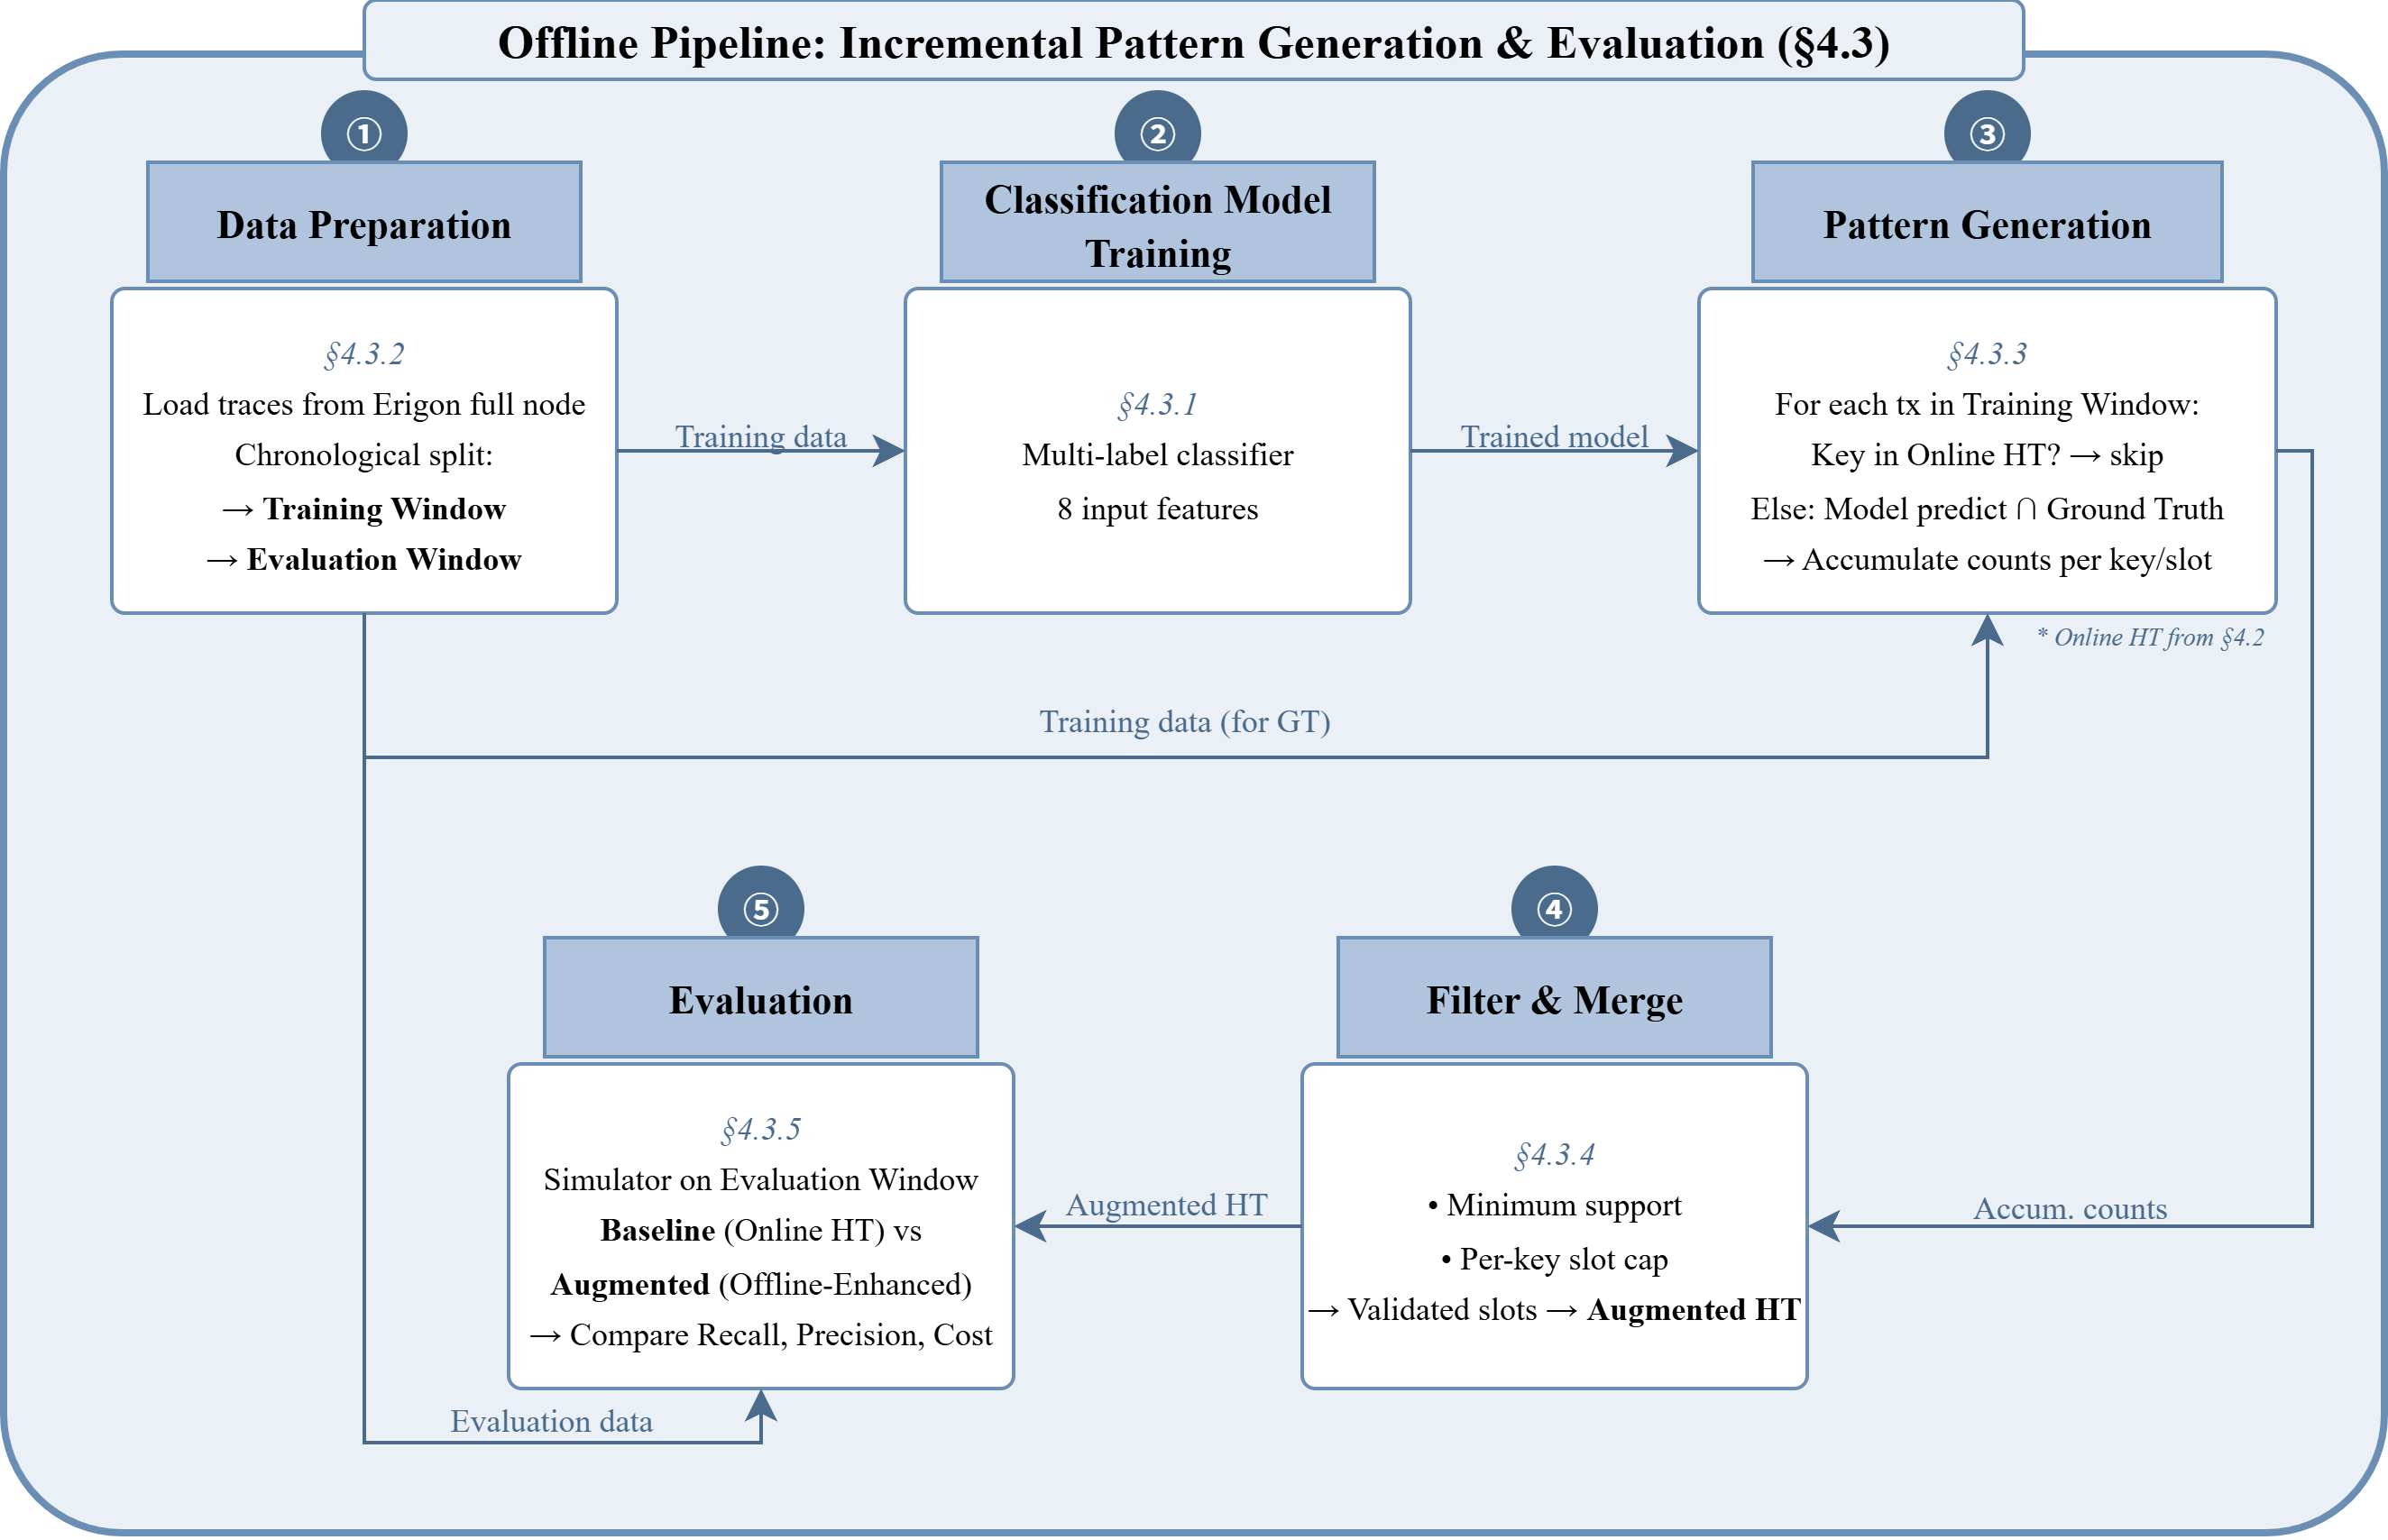
\includegraphics[width=0.95\columnwidth]{figures/system_design_pipeline.pdf}
\caption{Offline model training and evaluation pipeline.}
\label{fig:pipeline}
%\vspace{-0.5cm}
\end{figure}

For each transaction in the training window, the system checks whether its pattern key is stored in the online hash table. Stored keys are already covered and skipped; excluded keys invoke the classification model to produce a predicted slot set.

The predicted set from the model is then compared against the slots that the transaction actually accessed, as recorded in the training window. Let $\mathcal{P}(tx)$ denote the raw predicted slot set produced by the classification model for transaction $tx$, and $S_{\text{actual}}(tx)$ the set of slots that $tx$ actually accessed during execution (Equation~\ref{eq:union-size}). The intersection $\mathcal{P}(tx) \cap S_{\text{actual}}(tx)$ contains the slots that the model correctly predicted.
The result is a map $\mathcal{C}[k][s]$ that accumulates, for each pattern key $k$ and storage slot $s$, the number of transactions with key $k$ for which $s$ was correctly predicted. This accumulated count serves as a confidence measure: associations with low $\mathcal{C}[k][s]$ are likely coincidental and will be discarded by the minimum-support filter, while high-count associations represent reliable patterns worth merging into the hash table.

Transactions whose pattern key is excluded from the online hash table represent a significant fraction of all transactions.
Details are provided in Section~\ref{sec:evaluation}.

\begin{algorithm}[t]
\caption{Candidate Accumulation}
\label{alg:candidate-accum}
\begin{algorithmic}[1]
\Require Training window $\mathcal{W}_{\text{train}}$, online hash table $\mathcal{H}$, classification model $\mathcal{M}$
\Ensure Accumulated correct-prediction counts per pattern key and storage slot
\State Initialize an empty map $\mathcal{C}: \text{pattern\_key} \times \text{slot} \to \mathbb{N}$
\For{each transaction $tx$ in $\mathcal{W}_{\text{train}}$}
    \State Extract pattern key $k$ from $tx$
    \If{$k$ is stored in $\mathcal{H}$}
        \State \Comment{Covered by online path, skip}
    \Else
        \State Obtain predicted set $\mathcal{P} \gets \mathcal{M}(tx)$
        \State Obtain ground-truth set $S_{\text{actual}} \gets \text{actual slots accessed by }tx$
        \State $\mathcal{I} \gets \mathcal{P} \cap S_{\text{actual}}$
        \For{each slot $s$ in $\mathcal{I}$}
            \State $\mathcal{C}[k][s] \gets \mathcal{C}[k][s] + 1$
        \EndFor
    \EndIf
\EndFor
\State \Return $\mathcal{C}$
\end{algorithmic}
\end{algorithm}

\subsubsection{Filtering and Merging}
\label{sec:filtering-merging}

The accumulated counts $\mathcal{C}[k][s]$ from Algorithm~1 are the input to the filtering stage. Two criteria determine which slots are retained.

% 第一步：min_support 过滤。计数 < 阈值 → 噪声 → 丢弃。
\textbf{Minimum support.}
Only slots whose accumulated count $\mathcal{C}[k][s]$ exceeds a threshold $\tau_{\text{sup}}$ are retained.
This removes low-frequency noise that the model predicted correctly only by chance.

% 第二步：per-key slot 上限。按计数降序排列，优先保留高分 slot。
\textbf{Per-key slot limit.}
For each pattern key, the number of newly added slots is capped.
When the number of candidate slots exceeds the cap, those with higher counts take priority.
This prevents popular keys from bloating the hash table with many marginal predictions.

% 第三步：合并入 hash table。key 已存在 → 追加 slot；key 不存在 → 新建条目。
\textbf{Merge.}
After filtering, the remaining (pattern key, storage slot) pairs are merged into the online hash table.
If the pattern key already exists in the table, the new slots are appended to its existing set.
If the key is new, a new entry is created.
The augmented hash table uses the same key-value format as the original table, so online lookup remains $O(1)$ after the merge. Moreover, ML inference is incurred only during offline batch processing, and the pipeline supports continuous updates without any modification to the online path.
The effectiveness of this augmentation is evaluated in Section~\ref{sec:evaluation}.

% 这一部分直接删了，没有必要写在设计部分。
% \subsubsection{Evaluation}
% \label{sec:offline-evaluation}

% On the evaluation window, the same simulator is run twice: once with the baseline online hash table and once with the augmented hash table.
% Recall, precision, and total storage access cost are compared between the two configurations.
% Detailed results are presented in Section~\ref{sec:evaluation}.


\section{Evaluation}
\label{sec:evaluation}

\subsection{Implementation and Experimental Setup}

\subsubsection{Simulation Prototype}

To evaluate the prefetching strategy, we built a trace-driven offline replay simulator, avoiding the need to modify Erigon's codebase. Storage access traces are collected from an Erigon full node. The simulator replays these traces and applies the same intra-block cache semantics: cold accesses incur database lookup latency while hot accesses incur cache hit latency. The cache resets at each new block boundary, and prefetched slots are injected before execution begins. Since the access patterns are already recorded in the traces, the simulator captures the effect of prefetching without re-executing EVM bytecode.


\subsubsection{Experiment Configuration}
\label{sec:experiment-configuration}

Experiments are conducted on a machine with an Intel Core Ultra 9 285K processor (24 cores, \qty{5.1}{\giga\hertz}), \qty{128}{\giga\byte} of DDR5 memory, a \qty{3.6}{\tera\byte} NVMe SSD, and Ubuntu 22.04.5 LTS. The blockchain node is a modified Erigon client version 2.59. The software environment uses Python 3.10.12, LightGBM 4.6.0, and scikit-learn 1.7.2. Key hyperparameters are set as follows: the union threshold for hash table routing is $\theta = 152$, covering approximately 95\% of pattern keys, and the minimum support for candidate filtering is $\tau_{\text{sup}} = 2$. Cache latency parameters are based on empirical measurements on this hardware: cold access latency is \qty{3}{\micro\second} and hot access latency is \qty{30}{\nano\second}.

\subsubsection{Dataset}

Transaction execution traces are collected via the debug trace transaction interface for 1,001 consecutive Ethereum mainnet blocks from block height 20,000,000 to 20,001,000. After parsing, field normalization, and filtering, we obtain 94,463 valid transactions across 999 blocks (2 blocks contained no valid transactions after filtering and were excluded). The data is split chronologically at a 70\%/30\% ratio. The training window contains 699 blocks and 65,706 transactions. The evaluation window contains 300 blocks and 28,757 transactions.

\subsubsection{Experiment Groups}

The simulation platform supports four experimental settings, summarized in Table~\ref{tab:experiments}. E0 is the Erigon baseline without any prefetching. E1 is the oracle configuration, where predictions exactly equal ground-truth storage accesses. This configuration verifies simulator correctness and establishes the maximum potential benefit. E2 is SPML-PF without offline augmentation, which performs lookups using only the original pattern-key table. This measures the effectiveness of pure pattern-key-based prefetching. E3 is the full SPML-PF, which augments the hash table with patterns generated by the offline classification model. The offline model produces incremental patterns on the training window, which are filtered and merged into the online hash table without changing the $O(1)$ lookup interface.

The key distinction between E2 and E3 is the dictionary content: E2 uses the original pattern table built from historical transaction data, while E3 uses the table augmented with offline-generated patterns. Both share the same $O(1)$ hash table lookup mechanism.

\begin{table}[t]
\caption{Controlled experiment groups and their description.}
%\vspace{-0.5cm}
\label{tab:experiments}
\begin{center}
\begin{tabular}{cll}
\toprule
\textbf{Exp.} & \textbf{Prefetcher} & \textbf{Description} \\
\midrule
E0 & None & No-prefetch baseline \\
E1 & Oracle & Oracle upper bound \\
E2 & SPML-PF (w/o offline) & Original pattern-key table (baseline) \\
E3 & SPML-PF & Original + offline increments (proposed) \\
\bottomrule
\end{tabular}
\end{center}
%\vspace{-0.3cm}
\end{table}

\subsubsection{Evaluation Metrics}
\label{sec:eval-metrics}

Recall and precision are aggregated over all transactions following the definitions in Section~\ref{sec:problem-formulation} and computed over the evaluation window $\mathcal{W}_{\text{eval}}$. In addition, we report speedup as the total storage access cost of the E0 baseline divided by that of the evaluated scheme:

\begin{align}
\text{Recall} &= \frac{\sum_{tx \in \mathcal{W}_{\text{eval}}} |S_{\text{pred}}(tx) \cap S_{\text{actual}}(tx)|}{
\sum_{tx \in \mathcal{W}_{\text{eval}}} |S_{\text{actual}}(tx)|}, \nonumber \\
\text{Precision} &= \frac{\sum_{tx \in \mathcal{W}_{\text{eval}}} |S_{\text{pred}}(tx) \cap S_{\text{actual}}(tx)
|}{\sum_{tx \in \mathcal{W}_{\text{eval}}} |S_{\text{pred}}(tx)|}, \nonumber \\
\text{Speedup} &= \frac{\text{Cost}_{\text{E0}}}{\text{Cost}_{\text{scheme}}}.
\label{eq:eval-metrics}
\end{align}

\subsection{Performance Gains}

\subsubsection{Offline Augmentation Effect}

On the evaluation window, we compare SPML-PF without offline augmentation (E2) against the full SPML-PF (E3).

% 绘图脚本: evm_analysis/viz/plot_sim_figures.py / plot_main_results()
\begin{figure}[t]
\centering
\includegraphics[width=\columnwidth]{figures/main_results.pdf}
\caption{Accuracy and efficiency comparison of SPML-PF without offline augmentation (E2) and full SPML-PF (E3).}
\label{fig:main_results}
%\vspace{-0.2cm}
\end{figure}

% recall: 0.2223 -> 0.3117
We can observe from Fig.~\ref{fig:main_results}(a) that the recall metric improves by 40.2\%. The offline path discovers access patterns that the online hash table alone cannot cover. The offline pipeline adds 253 new pattern keys and 2,641 storage slots to the hash table, with an average of 10.4 slots per key.
Although precision drops by 12.7\%, which is a typical recall-precision trade-off, it is acceptable in practice because the savings from increased recall outweigh the cost of false positive prefetches.

% cost: (from 880,983~$\mu$s to 781,405~$\mu$s)
As shown in Fig.~\ref{fig:main_results}(b), total storage access cost decreases by 11.3\%. The recall gain dominates the cost of additional false positives. The speedup improves by 12.7\%, demonstrating that offline incremental patterns translate directly into online performance gains.

\subsubsection{Ablation Study}

E0 establishes the no-prefetch baseline. E1 establishes the theoretical upper bound. The gap between E0 and E1 defines the maximum room for improvement. E2 shows that the hash table alone captures 22.2\% of this gap. E3 (SPML-PF) further narrows the gap to 31.2\%, demonstrating that the offline-generated patterns provide additional coverage without changing the $O(1)$ lookup interface.

\subsection{Scaling Consistency}

To verify that the improvement generalizes across different transaction volumes, we repeat the experiment at three scales. The results are shown in Fig.~\ref{fig:scaling}.
Recall improvement of E3 over E2 grows monotonically with the dataset size, from +26.8\% at 2K transactions to +40.2\% at 94K transactions. Cost reduction follows the same trend, from -7.7\% at 2K transactions to -11.3\% at 94K transactions. Larger training windows provide richer historical signals for the offline classification model, leading to better generalization.

% \begin{table}[t]
% \caption{Scaling consistency analysis across three data sizes.}
% %\vspace{-0.2cm}
% \label{tab:scaling}
% \begin{center}
% \begin{tabular}{cccc}
% \toprule
% \textbf{Scale} & \textbf{Blocks} & \textbf{Recall Improvement} & \textbf{Cost Reduction} \\
% \midrule
% 2K txs & 23 & \textbf{+26.8\%} & \textbf{$-$7.7\%} \\  % 数据来源: evm_analysis/figures/data/scale_2k/rule_delta_eval.csv
% 10K txs & 115 & \textbf{+35.7\%} & \textbf{$-$10.9\%} \\  % 数据来源: evm_analysis/figures/data/scale_10k/rule_delta_eval.csv
% 94K txs & 999 & \textbf{+40.2\%} & \textbf{$-$11.3\%} \\  % 数据来源: evm_analysis/figures/data/rule_delta_eval.csv
% \bottomrule
% \end{tabular}
% \end{center}
% \end{table}

\begin{figure}[t]
\centering
\includegraphics[width=0.85\columnwidth]{figures/scaling_consistency_chart.pdf}
\caption{Scaling consistency analysis across three transaction volumes.}
\label{fig:scaling}
%\vspace{-0.2cm}
\end{figure}

\subsection{Parameter Sensitivity Analysis}

The cold access latency ($t_{\text{miss}}$) and hot access latency ($t_{\text{hit}}$) used in our simulator are measured empirically on our hardware platform. These values may differ across deployments. To verify that our conclusions are robust to variations in these parameters, we independently perturb each parameter by $\pm20\%$ and measure the resulting speedup values. Recall and precision are unaffected by latency parameters, as they depend solely on prediction correctness.

The results are shown in Table~\ref{tab:sensitivity}. The baseline row (default values) is shown in bold.
Both E2 and E3 speedups remain stable with a variation of only approximately $\pm0.1\%$ across all parameter combinations. This stability demonstrates that our method's performance is dominated by prediction accuracy, specifically which storage slots are prefetched, rather than by the exact latency values. As long as cold accesses are substantially more expensive than hot accesses, a condition that holds on any reasonable hardware configuration, the overall conclusion remains unchanged. The 100$\times$ gap between cold and hot access latencies is a general property of database-backed storage in blockchain clients, not an artifact of our specific measurements.

\begin{table}[t]
\caption{Parameter sensitivity analysis: E2 and E3 speedup under $\pm20\%$ perturbation of cold access ($t_{\text{miss}}$) and hot access ($t_{\text{hit}}$) latency.}
%\vspace{-0.5cm}
\label{tab:sensitivity}
\begin{center}
\begin{tabular}{cccc}
\toprule
\textbf{Parameters} & \textbf{E2 Speedup} & \textbf{E3 Speedup} & \textbf{Variation} \\
\midrule
\textbf{Baseline (\qty{30}{\nano\second} / \qty{3.0}{\micro\second})} & \textbf{1.2811$\times$} & \textbf{1.4444$\times$} & --- \\
$t_{\text{miss}}$ $-$20\% (\qty{30}{\nano\second} / \qty{2.4}{\micro\second}) & 1.2800$\times$ & 1.4423$\times$ & $\pm0.09\%$ \\
$t_{\text{miss}}$ $+$20\% (\qty{30}{\nano\second} / \qty{3.6}{\micro\second}) & 1.2819$\times$ & 1.4458$\times$ & $\pm0.10\%$ \\
$t_{\text{hit}}$ $-$20\% (\qty{30}{\nano\second} / \qty{3.0}{\micro\second}) & 1.2821$\times$ & 1.4461$\times$ & $\pm0.12\%$ \\
$t_{\text{hit}}$ $+$20\% (\qty{36}{\nano\second} / \qty{3.0}{\micro\second}) & 1.2802$\times$ & 1.4427$\times$ & $\pm0.09\%$ \\
\bottomrule
\end{tabular}
\end{center}
%\vspace{-0.5cm}
\end{table}


% \section{Limitation}
% \label{sec:limitation}

% This section discusses the limitations of our evaluation and identifies directions for improvement.

% First, simulation fidelity. Our simulator assumes perfectly timely prefetching. In a real deployment, prefetch requests may not complete before execution reaches the relevant storage load instruction. This means our results represent an upper bound on achievable benefits. A production implementation would need to account for prefetch scheduling and ensure that prefetched slots are ready before transaction execution begins.

% Second, I/O bandwidth contention. The current model does not account for additional I/O bandwidth consumed by inaccurate prefetches. Low-precision predictions cause unnecessary data movement that may compete with demand accesses. In a fully loaded system, this competition could reduce the effective throughput gain. Quantifying this effect requires integrating the prefetcher into a real client rather than using a trace-driven simulator.

% Third, empirical latency parameters. The cold access and hot access latencies are measured on our specific hardware configuration. Absolute speedup numbers may vary with different hardware, though the sensitivity analysis shows that the directional conclusions are stable across a $\pm20\%$ perturbation range.

% Fourth, dataset scope. The evaluation covers 1,001 consecutive Ethereum mainnet blocks, which is a representative sample but covers a limited time window. Contract usage patterns evolve over longer periods, potentially requiring periodic model retraining. The offline pipeline supports this retraining cycle, but the frequency of retraining and its impact on sustained performance remain to be studied.

% Fifth, model generalization. The offline classification model is trained on historical data from a specific block range. Drastic changes in contract usage patterns, such as new DeFi protocols or contract upgrades, may temporarily reduce prediction accuracy until the model is retrained on fresh data. Deploying the method in production would require monitoring prediction quality over time and triggering retraining when accuracy degrades below a threshold.


\section{Conclusion}
\label{sec:conclusion}

This paper addressed the performance bottleneck caused by cold storage slot accesses in the Ethereum Virtual Machine. We proposed a Split-Path ML-Augmented Prefetching method using an online/offline split-path architecture. The online path performs $O(1)$ hash table lookups with zero ML inference overhead. The offline path runs a classification model on historical data to generate incremental patterns that enhance the online hash table. This architecture decouples ML inference from the critical execution path, enabling continuous enhancement without online inference cost. Evaluated on 1,001 consecutive Ethereum mainnet blocks yielding approximately 94,000 transactions, SPML-PF improved recall from 22.23\% to 31.17\% (a 40.2\% relative increase) and reduced total storage access cost by 11.3\%. The recall gain grows monotonically with dataset size, achieving a 12.7\% overall speedup.

% Evaluated on 1,001 consecutive Ethereum mainnet blocks comprising approximately 94,000 transactions, recall improved from 22.23\% to 31.17\%, a relative improvement of 40.2\%. Total storage access cost was reduced by 11.3\%. The recall gain increases monotonically with data scale, demonstrating the scalability of the approach.

\bibliographystyle{IEEEtran}

\bibliography{references}

\vspace{12pt}

\end{document}
